\newcommand{\nomedoc}{Analisi Dei Requisiti}
\newcommand{\versione}{1.0}
\newcommand{\nomefile}{AnalisiDeiRequisiti-\versione.pdf}
\newcommand{\datacreazione}{6 Giugno 2011}
\newcommand{\datamodifica}{6 Giugno 2011}
\newcommand{\redazione}{Baron Federico}

% FUNZIONI TIPOGRAFICHE
\newcommand{\co}{\texttt} % courier
\newcommand{\bo}{\textbf} % bold
\newcommand{\pr}{\par\medskip} % paragrafo spaziato
\newcommand{\sca}{\textsc} % small caps

\documentclass[a4paper,12pt]{report}
% 10pt,11pt,12pt
% titlepage, notitlepage -> per dare inizio o no ad una nuova pagina dopo titolo
% twoside -> per dire se fronte-retro
\usepackage[latin1]{inputenc}
% per caratteri accentati
\usepackage[italian]{babel}
% per regole sintattiche italiane
\usepackage[bookmarks=true, pdfborder={0 0 0 0}]{hyperref}
% per collegamenti ipertestuali
\usepackage{graphicx}
% per inserimento immagini

% \usepackage{enumerate}
% per personalizzare elenchi puntati

\usepackage[hmargin=2cm]{geometry} %margine 2 cm
%\geometry{options varie}

% comandi per gestire meglio header e footer
\usepackage{fancyhdr}  % header e footer
\usepackage{totpages}
\pagestyle{fancy}
\renewcommand{\headrulewidth}{0.4pt}
\renewcommand{\footrulewidth}{0.4pt}

\setlength{\headheight}{1.2cm} % NON TOCCARE
\setlength{\voffset}{-1.5cm} % NON TOCCARE
\setlength{\textheight}{666pt} % NON TOCCARE
\setlength{\footskip}{60pt}
\setlength{\parindent}{0pt} % INDENTAZIONE

\lhead{\nomedoc\  (ver. \versione)}
\chead{}
\rhead{
\includegraphics[height=1cm]{img/netmus.png}}
\lfoot{
\includegraphics[height=0.8cm]{img/logo.png}}
\cfoot{}
\rfoot{\thepage}

\usepackage{titlesec}
\titleformat{\chapter}{\normalfont\huge\bfseries}
{\thechapter}{20pt}{\Huge}

\usepackage{rotating}   % PER TABELLE E AMBIENTI RUOTATI
\usepackage{array}
\usepackage{color}
\usepackage{colortbl}  % VARIE PER GESTIRE I COLORI
\definecolor{Orange}{RGB}{255,127,0}   % ARANCIO ACCES0
\definecolor{orange}{RGB}{255,207,80}  % ARANCIO TENUE

\addtocontents{toc}{\protect\thispagestyle{fancy}}  % PER INDICI CON + PAGINE
\usepackage[font=it]{caption}    % PER RENDERE CORSIVE LE DIDASCALIE
\usepackage{eurosym}  % PER SIMBOLO EURO

% \usepackage{listings}   per codice sorgente

\author{VT.G - Valter Texas Group}

\begin{document}

\pagenumbering{Roman} % INIZIO NUMERAZIONE ARABA

\vspace*{1cm}
\begin{center}

\begin{LARGE} \sca{Federico Baron} \end{LARGE}\\
\vspace{0.5cm}
\begin{Large}
\emph{fede.baron.89@gmail.com} \end{Large}\\
\vspace*{1cm} 
\includegraphics[width=5cm]{img/logo.png}\\
\vspace{0.5cm}
\begin{Large} \emph{``Comunicazione Aumentata/Alternativa per Giovani Ospiti
della Terapia Intensiva Pediatrica''} \end{Large}\\
\vspace{3cm}
\begin{Large} \sca{\nomedoc} \end{Large}\\
\end{center}
\vspace{1cm}

% INFORMAZIONI DOCUMENTO
\begin{center}
\begin{tabular}{r|l}
\hline & \\
\bo{Nome} & \nomefile \\
\bo{Versione attuale} & \versione \\
\bo{Data creazione} & \datacreazione \\
\bo{Data ultima modifica} & \datamodifica \\
\bo{Redazione} & \redazione \\
& \\\hline
\end{tabular}
\end{center}
\newpage

\chapter*{Sommario}
\thispagestyle{fancy}
Nel presente documento vengono individuati ed elencati i requisiti che verranno
soddisfatti nello sviluppo del software. ecc ecc\ldots

% INDICE
\tableofcontents

\chapter{Introduzione}
\thispagestyle{fancy} % serve perche' nelle pagine di inizio Chapter esca header e footer
\pagenumbering{arabic} % INIZIO NUMERAZIONE NORMALE
\rfoot{\thepage\ di \pageref{TotPages}}

\section{Scopo del documento}
Il presente documento ha lo scopo di presentare al committente l'Analisi dei
Requisiti e le potenzialit\`a del nostro prodotto software per soddisfare le
richieste del capitolato d'appalto C02 NetMus (vedi 1.4.2 - Riferimenti
Normativi).


\section{Scopo del prodotto}
Il progetto \underline{NetMus} nasce con lo scopo di realizzare un sistema
software basato su \underline{cloud} \underline{computing}, per memorizzare
informazioni di brani musicali in profili utente online.\\ Tali informazioni vengono estratte da
dispositivi musicali o di archiviazione \underline{USB} al momento della loro connessione.

\section{Glossario}
Il Glossario \`e definito con un documento a parte
(\emph{Glossario-\versioneglossario.pdf}). Tutti i termini caratterizzati da
\underline{questa sottolineatura} sono ivi definiti.\\
Verr\`a sottolineata solamente la prima occorrenza di ciascun
termine presente nel Glossario, per non compromettere la leggibilit\`a del documento.

\section{Riferimenti}

\subsection{Normativi} % oppure rif. a Norme di progetto con leggi e tutto
\begin{itemize}
  \item ISO/IEC 12207:1995 - Cicli di vita software
  \item ISO/IEC 9126:2001 - Quality Model
  \item \emph{NormeDiProgetto-\versionenormeprogetto.pdf} che regola e
  accompagna tutti i documenti ufficiali.
\end{itemize}
\newpage
\subsection{Informativi}
\begin{itemize}
  \item Capitolato d'appalto CO2-NETMUS del corso di Ingegneria del Software
  A.A. 2010/11 :\\
  \url{http://www.math.unipd.it/~tullio/IS-1/2010/Progetto/NetMus.pdf}
  \item Slide delle lezioni del corso:\\
  \url{http://www.math.unipd.it/~tullio/IS-1/2010/}
  \item Verbale intervista proponente:\\
  \co{allegato Verbale-1.0.pdf}
  \item Sistema di cloud Google App Engine:\\
  \url{http://code.google.com/intl/it/appengine/}
\end{itemize}


% INIZIO CAPITOLO 2
\chapter{Descrizione generale}
\thispagestyle{fancy}

\section{Contesto d'uso del prodotto}
Il progetto che ho intenzione di sviluppare \`e un software
destinato ad una fascia d'utenza ristretta. In particolare l'utilizzo avverrà da
parte di bambini e ragazzi ospiti in un reparto di terapia intensiva e dai loro
parenti e dal personale ospedaliero che avranno la necessità di configurare lo
strumento secondo le specifiche esigenze.

\subsection{Piattaforma d'esecuzione e interfacciamento con l'ambiente di
installazione e uso}
Tablet Android(>2.3) e iPad!

\section{Caratteristiche degli utenti}
Gli utenti, in molti casi, non avranno conoscenze informatiche e non avranno
esperienza sull'utilizzo di strumenti tablet. Inoltre i bambini ricoverati che
utilizzeranno questo strumento, a causa di patologie temporanee/permanenti o
dell'età, potrbebero avere delle difficoltà di movimento degli arti superiori e
dei difetti cognitivi e di vista.

\section{Assunzioni e dipendenze}
Tablet Android >2.3 e iPad > boh.

\chapter{Use case}
\thispagestyle{fancy}

% \section{UC1- Titolo}
% \begin{figure}[h]
%   \centering
%   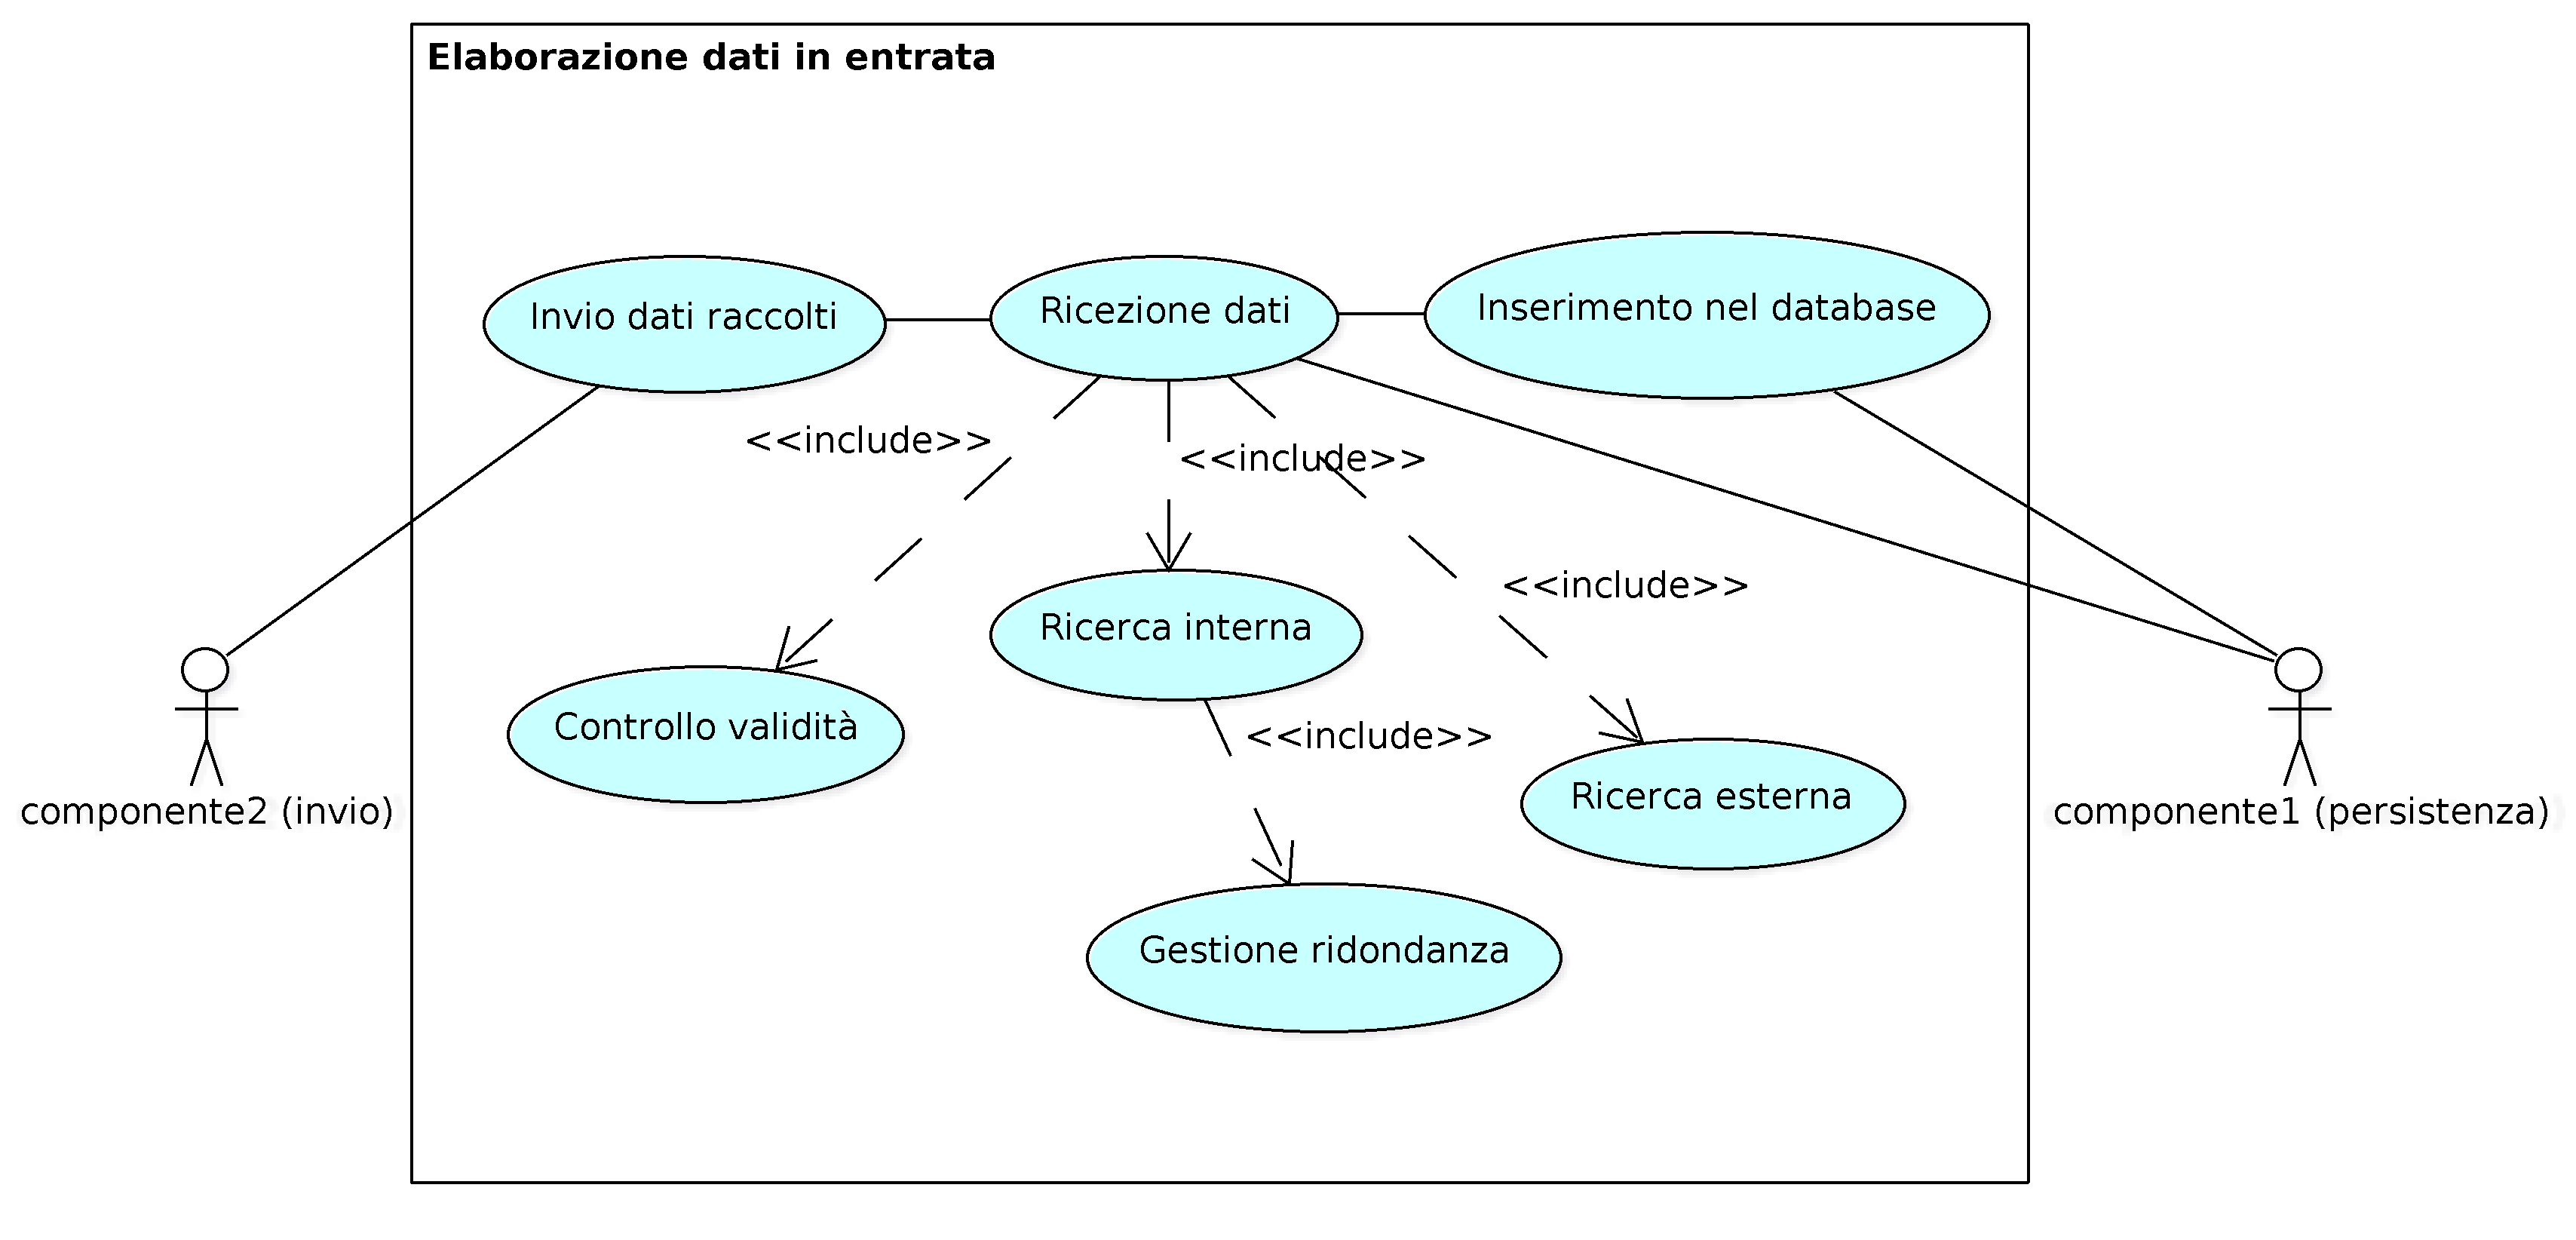
\includegraphics[width=10cm]{img/AR/UC2_2.png}
% \caption{}
% \end{figure}

\vspace*{0.5cm}
\bo{Use case UC1: Titolo} \\\\
\bo{Attori primari:} \\\\ 
\bo{Pre-condizioni:} \\\\
\bo{Post-condizioni:} \\\\
\bo{Scenario principale:}
\begin{enumerate}
  \item 1
  \item 2
\end{enumerate}
\bo{Scenari secondari:}
\begin{itemize}
  \item scenario secondario 1
  \begin {enumerate}
    \item 1
  \end{enumerate}
\end{itemize}
\newpage


\chapter{Lista dei requisiti}
\thispagestyle{fancy}

\section{Requisiti funzionali}

\subsection*{Applicazione equivalente allo strumento cartaceo già in uso}
\bo{Tipo:} funzionale \\
\bo{Richiesta:} obbligatorio \\
L'applicazione deve garantire almeno le funzionalità, oppurtunamente
digitalizzate, presenti nello strumento cartaceo da cui prende spunto. Questo
strumento consiste in un libretto sfogliabile con una figura rappresentante uno
stato/bisgono per ogni pagina.

\subsection*{Visualizzare la sequenza di immagini standard}
\bo{Tipo:} funzionale \\
\bo{Richiesta:} obbligatorio \\
L'utente deve poter navigare avanti e indietro nella lista delle immagini
standard ottenute dallo strumento cartaceo.

\subsection*{Selezionare una delle immagini}
\bo{Tipo:} funzionale \\
\bo{Richiesta:} obbligatorio \\
Mentre si visualizza un'immagine questa puo' essere scelta nel modo pi\`u
semplice possibile.

\subsection*{Ordine delle immagini}
\bo{Tipo:} funzionale \\
\bo{Richiesta:} desiderabile \\
L'ordine delle immagini proposte viene ottimizzato in base alla frequenza di
selezione nelle sessioni passate.

\section{Requisiti di qualit\`a}

\subsection*{Nome requisito}
\bo{Id:} id \\
\bo{Tipo:} qualità \\
\bo{Richiesta:} obbligatorio \\
Descrizione.

\section{Requisiti di vincolo}

\subsection*{Nome requisito}
\bo{Id:} id \\
\bo{Tipo:} vincolo \\
\bo{Richiesta:} obbligatorio \\
Descrizione.

% \newpage
% \subsection{Gerarchia dei requisiti}
% 
% \begin{table}[!h]
% \centering
% \begin{footnotesize}
% \begin{tabular}{|l|l|}
% 
% \rowcolor{Orange}
% \bo{Web Application Netmus} \\
% \hline
% \cellcolor{orange}
% Grafica simile ad iTunes & Elenco brani raggruppati opportunamente \\
% & Menu laterali \\   
% & Visualizzazione informazioni dettagliate di un brano \\         
% & Visualizza player YouTube \\         
% \hline
% \cellcolor{orange}
% Creazione profilo utente tramite registrazione & Pagina di login dipendente da Google login \\ 
% \hline
% \cellcolor{orange}
% Personalizzazione del proprio catalogo & Cancellazione brano \\
% & Modifica informazioni brano \\       
% & Creazione playlist \\
% & Ranking brani \\   
% \hline
% \cellcolor{orange}
% Gestione profilo personale & Modifica informazioni personali \\         
% & Cambio password \\
% & Cancellazione del proprio account \\       
% & Pubblicazione profilo \\
% \hline
% \cellcolor{orange}
% Riproduzione tracce in streaming & Ottimizzazione della ricerca su YouTube \\       
% & Quote YouTube \\
% & YouTube Terms of Service \\       
% \hline
% \cellcolor{orange}
% Scalabilit\`a & Scalabilit\`a di interfaccia grafica \\       
% & Scalabilit\`a di massa d'utenza \\   
% \hline
% \cellcolor{orange}
% Interazione con altri utenti & Visualizzazione di altri profili \\        
% & Lasciare commenti su altri profili \\         
% \hline
% \cellcolor{orange}
% Elaborazione dati utente & Esportazione pdf \\
% \hline
% \cellcolor{orange}
% Ricezione ed elaborazione brani & Controllo di validit\`a dati \\   
% & Controllo informazioni da database interno \\       
% & Identificazione di dati ridondanti \\
% & Inserimento nel database \\
% & Gestione concorrenza \\
% & Completamento informazioni da servizio esterno \\         
% \hline
% \cellcolor{orange}
% Invio nuove informazioni a Componente 2& \\       
% \hline
% \cellcolor{orange}
% Deve utilizzare il cloud computing& \\
% \hline
% \cellcolor{orange}
% Deve utilizzare tecnologie GAE e GWT& \\
% \hline
% \cellcolor{orange}
% Gestione database & Deve utilizzare Google Datastore \\        
% \hline
% \end{tabular}
% \\\vspace{1cm}
% \begin{tabular}{|l|}
% \hline
% \rowcolor{Orange}
% \bo{Utilizzo} \\
% \hline
% \rowcolor{orange}
%  Accessibilit\`a \\
%  \rowcolor{orange}                  
%  Open source \\  
%  \rowcolor{orange}         
%  Portabilit\`a \\
%  \rowcolor{orange}               
%  Sviluppo multi-lingua \\
%  \rowcolor{orange}                  
%  Semplicit\`a di utilizzo \\
%  \rowcolor{orange}               
%  Manutenibilit\`a \\
%  \rowcolor{orange}         
%  Gestione errori \\             
% \hline
% \end{tabular}
% \hspace{3cm}
% \begin{tabular}{|l|}
% \hline
% \rowcolor{Orange}
% \bo{Documenti} \\           
% \hline
% \rowcolor{orange}
%  Manuale utente \\                 
% \hline
% \rowcolor{orange}
%  Manuale utente inglese \\                  
% \hline
% \end{tabular}
% \end{footnotesize}
% \caption{Gerarchia dei requisiti (C1)}
% \end{table}
% 
% \begin{sidewaystable}[]
% \centering
% \begin{footnotesize}
% \begin{tabular}{|l|l|l|}
% \rowcolor{Orange}
% \bo{Requisiti Funzionali}\\
% \hline
% \rowcolor{orange}                         
% \sca{Necessari} & \sca{Desiderabili} & \sca{Opzionali} \\         
% C1FN-1 Web Application Netmus & C1FD-1.1.4 Visualizza player YouTube &
% C1FO-1.2.1 Pagina login indipendente \\
% C1FN-1.1 Grafica simile ad iTunes & C1FD-1.3 Personalizzazione del catalogo & C1FO-1.3.3 Creazione playlist \\
%  C1FN-1.1.1 Brani elencati opportunamente & C1FD-1.3.1 Cancellazione brano & C1FO-1.3.4 Ranking brani \\ 
% C1FN-1.1.2 Menu laterali & C1FD-1.3.2 Modifica informazioni brano & C1FO-1.7.2
% Lasciare commenti su  \\ C1FN-1.1.3 Visualiz. info dettagliate dei brani & C1FD-1.4.4 Pubblicazione
% profilo & C1FO-1.8.1 Esportazione PDF \\ C1FN-1.4 Gestione profilo personale &
% C1FD-1.5 Riproduzione tracce in streaming & C1FO-1.9.3 Completamento info da  \\
% C1FN-1.4.1 Modifica informazioni personali & C1FD-1.7 Interazione con altri utenti & \\       
% C1FN-1.4.3 Cancellazione del proprio account & C1FD-1.7.1 Visualizzazione altri profili & \\                    
% C1FN-1.9 Ricezione ed elaborazione dei brani & C1FD-1.8 Elaborazione dati utente &   \\             
% C1FN-1.9.1 Controllo di validit\`a dei dati & C1FD-1.10 Invio nuove informazioni a C2 & \\                
% C1FN-1.9.2 Completamento info da database interno & & \\                                                         
% C1FN-1.9.5 Inserimento nel Database & & \\                             
% C1FN-1.13 Gestione Database &  & \\                   
% \hline
% \end{tabular}
% \caption{Requisiti funzionali (C1)}
% 
% \begin{tabular}{|l|l|l|}
% \cline{1-1}
% \rowcolor{Orange}
% \bo{Requisiti Di Qualit\`a} \\
% \hline
% \rowcolor{orange}                         
% \sca{Necessari} & \sca{Desiderabili} & \sca{Opzionali} \\
% C1QN-1.6 Scalabilit\`a & C1QD-1.5.1 Ottimizzazione della ricerca su YouTube &
% C1QO-2.1 Accessibilit\`a   \\ C1QD-1.6.1 Scalabilit\`a interfaccia grafica &
% C1QD-2.4 Supporto multilingua & \\ C1QN-1.6.2 Scalabilit\`a massa di utenza  &
% C1QD-3.1.1 Manuale utente inglese & \\ C1QN-1.9.4 Identificazione dati ridondanti & & \\                          
% C1QN-1.9.6 Gestione concorrenza &  & \\                          
% C1QN-2.3 Portabilit\`a &  & \\              
% C1QN-2.7 Gestione errori &  &   \\       
% C1QN-3.1 Manuale utente &  & \\                            
% \hline
% \end{tabular}
% \caption{Requisiti di qualit\`a (C1)}
% \end{footnotesize}
% \end{sidewaystable}
% 
% % requisiti di vincolo
% 
% \begin{table}
% \centering
% \begin{footnotesize}
% \begin{tabular}{|l|l|l|}
% \cline{1-1}
% \rowcolor{Orange}
% \bo{Requisiti Di Vincolo}   \\
% \hline
% \rowcolor{orange}                         
% \sca{Necessari} & \sca{Desiderabili} \\   
% C1VN-1.12 Deve utilizzare tecnologie GAE e GWT & C1VD-1.5.2 Quote YouTube   \\ 
% C1VN-1.13.1 Deve utilizzare Google Data Store & C1VD-1.5.3 YouTube Terms of
% Services \\
% C1VN-1.11 Deve utilizzare il cloud computing & \\  
% C1VN-2.2 Open source & \\
% C1VN-2.5 Semplicit\`a di utilizzo & \\
% \hline
% \end{tabular}
% \caption{Requisiti di vincolo (C1)}
% \end{footnotesize}
% \end{table}
% 
% \newpage
% 
% %---------------
% 
% \chapter{Tracciamento dei requisiti}
% \thispagestyle{fancy}
% 
% \section{Tracciamento requisiti - use case}
% \begin{footnotesize}
% \centering
% \begin{longtable}[!h]{|l|l|}
% \hline
% \rowcolor{orange}                         
% \sca{Requisiti} & \sca{Use case}\\
% \hline
% \endhead
% \hline
% \multicolumn{2}{|c|}{\textit{continua alla pagina successiva}}\\
% \hline
% \endfoot
% \endlastfoot
% C1FN-1.1 Grafica simile ad iTunes & UC1.3.1 - Visualizzare catalogo \\ 
% & UC1.3.3.1 - Visualizzare dettagli brano \\
% & UC1.2.1 - Visualizzare catalogo di altri utenti \\
% & UC1.2.3 - Visualizzare profilo di altri utenti \\\hline
% C1FN-1.1.1 Brani elencati opportunamente & UC1.3.1 - Visualizzare catalogo \\
% \hline
% C1FN-1.1.2 Menu laterali & UC1.3.1 - Visualizzare catalogo \\ \hline
% C1FN-1.1.3 Visualiz. info dettagliate dei brani & UC1.3.3.1 - Visualizzare dettagli brano \\ \hline
% C1FD-1.1.4 Visualizza player YouTube & UC1.3.3.2 - Player YouTube \\ \hline
% C1FN-1.2 Registrazione & UC1.4.2 - Registrazione NetMus \\ \hline
% C1FO-1.2.1 Pagina login indipendente & UC1.4 - Autenticazione \\
% & UC1.4.3  - Autenticazione NetMus \\ 
% & UC1.4.1 - Registrazione Google \\ \hline
% C1FD-1.3 Personalizzazione del catalogo & UC1.3 - Gestire libreria musicale \\
% & UC1.3.2 - Modificare informazioni catalogo \\
% \hline 
% C1FD-1.3.1 Cancellazione brano & UC1.3.3 - Gestire dettagli brano \\ \hline
% C1FD-1.3.2 Modifica informazioni brano & UC1.3.3.3 - Modificare informazioni
% brano \\ \hline 
% C1FO-1.3.3 Creazione playlist & UC1.3.5 - Creare playlist \\ \hline 
% C1FO-1.3.4 Ranking brani & UC1.3.2 - Modificare informazioni catalogo \\ \hline 
% C1FN-1.4 Gestione profilo personale & UC1.1 - Gestire profilo personale \\
% \hline 
% C1FN-1.4.1 Modifica informazioni personali & UC1.1.3 - Modificare informazioni
% profilo \\ \hline
% C1FN-1.4.2 Cambio password & UC1.1.3 - Modificare informazioni
% profilo \\ \hline
% C1FN-1.4.3 Cancellazione del proprio account & UC1.1.1 - Cancellare profilo \\
% & UC1.1.4 - Cancellare catalogo \\ \hline
% C1FD-1.4.4 Pubblicazione profilo & UC1.1.2 - Pubblicare profilo \\
% & UC1.1.5 - Pubblicare a tutti \\
% & UC1.1.6 - Pubblicare a selezione \\ \hline
% C1FD-1.5 Riproduzione tracce in streaming & UC1.3.3.2 - Player YouTube \\ \hline
% C1FD-1.7 Interazione con altri utenti & UC1.2 - Interagire con altri cataloghi
% \\ \hline 
% C1FD-1.7.1 Visualizzazione altri profili & UC1.2.3 - Visualizzare profilo
% di altri utenti \\
% & UC1.2.1 - Visualizzare catalogo di altri utenti \\ \hline
% C1FO-1.7.2 Lasciare commenti su profilo & UC1.2.2 - Scrivere commenti \\ \hline
% C1FO-1.8.1 Esportazione PDF & UC1.3.4 - Esportare pdf \\ \hline
% C1FD-1.10 Invio nuove informazioni a C2 & UC2.1 - Aggiornamento informazioni \\
% \hline
% %requisiti c2
% C2FN-1 Recupero delle informazioni & UC2.2 - Inviare nuovi brani \\
% \hline
% C2FN-1.1 Recupero automatico & UC2.2.1 - Invio automatico \\ \hline
% C2FN-1.2 Recupero manuale & UC2.2.2 - Invio manuale \\ \hline
% C2FD-1.4 Informazioni dall'hard disk & UC2.2 - Inviare nuovi brani \\
% \hline
% C2FN-1.5 File ignorati & UC2.2 - Inviare nuovi brani \\ \hline
% C2FD-2 Aggiornamento e completamento informazioni & UC2.1 Aggiornamento
% informazioni \\ \hline 
% C2FN-3 Comunicazione con C1 & UC2.2 - Inviare nuovi brani \\
% & UC2.1 - Aggiornamento informazioni \\ \hline 
% C2FN-3.1 Invio delle informazioni & UC2.2 - Inviare nuovi brani \\
% \hline
% \caption{Tracciamento requisiti - use case}
% \end{longtable}
% \end{footnotesize}
% 
% \section{Tracciamento use case - requisiti}
% 
% \begin{footnotesize}
% \centering
% \begin{longtable}[!h]{|l|l|}
% \hline
% \rowcolor{orange}                         
% \sca{Use case} & \sca{Requisiti} \\
% \hline
% \endhead
% \hline
% \multicolumn{2}{|c|}{\textit{continua alla pagina successiva}}\\
% \hline
% \endfoot
% \endlastfoot
% UC1.1 - Gestire profilo personale & C1FN-1.4 Gestione profilo personale \\
% \hline
% UC1.1.1 - Cancellare profilo & C1FN-1.4.3 Cancellazione del proprio account \\
% \hline
% UC1.1.2 - Pubblicare profilo & C1FD-1.4.4 Pubblicare profilo \\ \hline
% UC1.1.5 - Pubblicare a tutti & C1FD-1.4.4 Pubblicare profilo \\ \hline
% UC1.1.6 - Pubblicare a selezione & C1FD-1.4.4 Pubblicare profilo \\ \hline
% UC1.1.3 - Modificare informazioni profilo & C1FN-1.4.1 Modifica informazioni
% personali \\ 
% & C1FN-1.4.2 Cambio password \\ \hline
% UC1.1.4 - Cancellare catalogo & C1FN-1.4.3 Cancellazione del proprio account \\
% \hline 
% UC1.2 - Interagire con altri cataloghi & C1FD-1.7 Interazione con altri utenti
% \\ \hline
% UC1.2.1 - Visualizzare catalogo di altri utenti & C1FD-1.7.1 Visualizzazione
% altri profili \\ 
% & C1FN-1.1 Grafica simile ad iTunes \\ \hline 
% UC1.2.2 - Scrivere commenti & C1FO-1.7.2 Lasciare commenti su profilo \\ \hline
% UC1.2.3 - Visualizzare profilo di altri utenti & C1FN-1.1 Grafica simile ad
% iTunes \\ 
% & C1FD-1.7.1 Visualizzazione altri profili \\ \hline
% UC1.3 - Gestire libreria musicale & C1FD-1.3 Personalizzazione del catalogo \\
% \hline
% UC1.3.1 - Visualizzare catalogo & C1FN-1.1 Grafica simile ad iTunes \\
% & C1FN-1.1.1 Brani elencati opportunamente \\
% & C1FN-1.1.2 Menu laterali \\ \hline
% UC1.3.2 - Modificare informazioni catalogo & C1FD-1.3 Personalizzazione del
% catalogo \\ 
% & C1FO-1.3.4 Ranking brani \\ \hline
% UC1.3.3 - Gestire dettagli brano & C1FD-1.3.1 Cancellazione brano \\ \hline
% UC1.3.3.1 - Visualizzare dettagli brano & C1FN-1.1 Grafica simile ad iTunes \\
% & C1FN-1.1.3 Visualiz. info dettagliate dei brani \\ \hline
% UC1.3.3.2 - Player YouTube & C1FD-1.1.4 Visualizza player YouTube \\
% & C1FD-1.5 Riproduzione tracce in streaming \\ \hline
% UC1.3.3.3 - Modificare informazioni brano & C1FD-1.3.2 Modifica informazioni
% brano \\ \hline
% UC1.3.4 - Esportare pdf & C1FO-1.8.1 Esportazione PDF \\ \hline
% UC1.3.5 - Creare playlist & C1FO-1.3.3 Creazione playlist \\ \hline 
% UC1.4 - Autenticazione & C1FO-1.2.1 Pagina login indipendente \\ \hline
% UC1.4.1 - Registrazione Google & C1FO-1.2.1 Pagina login indipendente \\ \hline
% UC1.4.2 - Registrazione NetMus & C1FN-1.2 Registrazione \\ \hline
% UC1.4.3  - Autenticazione NetMus & C1FO-1.2.1 Pagina login indipendente \\
% \hline
% UC2.1 - Aggiornamento informazioni & C1FD-1.10 Invio nuove informazioni a C2 \\
% & C2FD-2 Aggiornamento e completamento informazioni \\
% & C2FN-3 Comunicazione con C1 \\ \hline
% UC2.2 - Inviare nuovi brani & C2FN-1 Recupero delle informazioni \\
% & C2FD-1.4 Informazioni dall'hard disk \\
% & C2FN-1.5 File ignorati \\
% & C2FN-3 Comunicazione con C1 \\
% & C2FN-3.1 Invio delle informazioni \\ \hline
% UC2.2.1 - Invio automatico & C2FN-1.1 Recupero automatico \\ \hline
% UC2.2.2 - Invio manuale & C2FN-1.2 Recupero manuale \\ \hline
% \caption{Tracciamento use case - requisiti}
% \end{longtable}
% \end{footnotesize}
% 
% 
% \section{Requisiti non tracciati}
% 
% I requisiti qui elencati non sono stati tracciati da alcun Use Case, questo in
% quanto i requisiti di vincolo e di qualit\`a non sono rappresentabili da nessuno
% di essi ma sorgono dalle richieste del capitolato o da regole di buon sviluppo
% di un progetto di Ingegneria del Software.
% Gli altri vincoli funzionali, come ad esempio C1FN-1.13 Gestione Database, non sono
% tracciati in quanto esprimono funzioni che non si potrebbero evincere da alcuno Use
% Case ma riguardano piuttosto elementi strutturali del sistema NetMus.
% 
% 
% \begin{table}[!htpb]
% \centering
% \begin{footnotesize}
% \begin{tabular}{|l|}
% \cline{1-1}
% \rowcolor{orange}
% \hline
% \bo{Requisiti non tracciati} \\
% \hline
% C1FN-1 Web Application Netmus \\ \hline
% C1QD-1.5.1 Ottimizzazione della ricerca su YouTube \\ \hline
% C1VD-1.5.2 Quote YouTube \\ \hline
% C1VD-1.5.3 YouTube Terms of Services \\ \hline
% C1QN-1.6 Scalabilit\`a \\ \hline
% C1QN-1.6.1 Scalabilit\`a interfaccia grafica \\ \hline
% C1QN-1.6.2 Scalabilit\`a massa di utenza \\ \hline
% C1FD-1.8 Elaborazione dati utente \\ \hline
% C1FN-1.9 Ricezione ed elaborazione dei brani \\ \hline
% C1FN-1.9.1 Controllo di validit\`a dei dati \\ \hline
% C1FN-1.9.2 Completamento info da database interno \\ \hline
% C1FO-1.9.3 Completamento info da servizio esterno \\ \hline
% C1QN-1.9.4 Identificazione dati ridondanti \\ \hline
% C1FN-1.9.5 Inserimento nel Database \\ \hline
% C1QN-1.9.6 Gestione concorrenza \\ \hline
% C1VN-1.11 Deve utilizzare il cloud computing \\ \hline
% C1VN-1.12 Tecnologie GAE e GWT \\ \hline
% C1FN-1.13 Gestione Database \\ \hline
% C1VN-1.13.1 Deve utilizzare Google Data Store \\ \hline
% C1QN-2 Utilizzo \\ \hline
% C1QO-2.1 Accessibilit\`a \\ \hline
% C1VN-2.2 Open source \\ \hline
% C1QN-2.3 Portabilit\`a \\ \hline
% C1QD-2.4 Supporto multi-lingua \\ \hline
% C1VN-2.5 Semplicit\`a di utilizzo \\ \hline
% C1QN-2.6 Manutenibilit\`a \\ \hline
% C1QN-2.7 Gestione errori \\ \hline
% C1QN-3.1 Manuale utente \\ \hline
% C1QD-3.1.1 Manuale utente inglese \\ \hline
% %c2
% C2FO-1.3 Informazioni senza connessione \\ \hline
% C2FO-1.6 Indicazioni file ignorati \\ \hline
% C2QD-1.7 Ottimizzazione memoria cache \\ \hline 
% C2QN-3.2 Utilizzo della connessione \\ \hline
% C2QN-4 Utilizzo \\ \hline 
% C2QD-4.1 Portabilit\`a \\ \hline
% C2QD-4.2 Semplicit\`a di utilizzo \\ \hline
% C2QD-4.3 Supporto multi-lingua \\ \hline
% C2QN-4.4 Manutenibilit\`a \\ \hline
% C2VD-4.5 Meno disturbo possibile \\ \hline
% C2VN-4.6 Norme legali \\ \hline
% C2VN-4.7 Open source \\ \hline
% \end{tabular}
% \end{footnotesize}
% \caption{Requisiti non tracciati}
% \end{table}


\listoftables
\addcontentsline{toc}{chapter}{Indice Tabelle}
\listoffigures
\addcontentsline{toc}{chapter}{Indice Figure}
\end{document}

